
\chapter{Background}
\label{chapter2}

% 2.1
\section{Magnetohydrodynamics}


The term ``magnetohydrodynamics'' (MHD) is a portmanteau of two physical concepts which are used to model plasmas 
inside fusion reactors (among other things): the ``\textbf{m}agneto'' term comes from ``magnetic field'', and ``\textbf{h}ydro\textbf{d}ynamics'' indicates a 
a fluid dynamics component. Put together, magnetohydrodynamics is the study of electrically conductive materials 
that behave like fluids. Essentially it provides a way to model the behaviour of a (considerably volumous!) 
mass of conductive particles, and their electrodynamic forces, as if it were a fluid, as opposed to having to model 
individual particle interactions. This idea was first introducd by Hannes Alfv\'en in 1970, for which he earned 
the Nobel prize \cite{alfven-mhd}!

Much modern research in Tokamak plasma simulation uses some variation of an MHD model (and the derived Grad-Shafranov Equation, which we will 
soon be introduced to) for a number of reasons, not least being its comparative computational efficiency.
One primary benefit of treating our plasma as a fluid being that we avoid modelling the behaviour of 
each individual particle in said plasma, a simplification which becomes especially important when we consider 
the order of number of particles we would have to simulate is of order $\sim 10^{20}$ - far too much 
for the author's ThinkPad T440p to even contemplate!

Here we will build the relevant MHD background for this thesis, deriving the MHD equations from first principles, 
and explaning the assumptions we make to reduce them to a simplified state known as ``ideal MHD''. From there we will 
look at the PDE which models the behaviour of a plasma inside a Tokamak, the ``Grad-Shafranov Equation''. We will 
then note some pitfalls of using this model to describe AC configuration Tokamaks (as we are investigating), 
and finish with a discussion on runaway electrons (RE).

% 2.1.1.
\subsection{MHD Theory}

Given MHD is the marriage of fluid dynamics with electrodynamics, it is only natural to begin our 
study looking at the equations which describe electrodynamic behaviour --- Maxwell's equations 
describe the interaction between magnetic fields $\vec{B}(\vec{r}, t)$, electric fields $\vec{E}(\vec{r}, t)$, and 
the current density $j(\vec{r}, t)$ which induces them, where $\vec{r} \in \R^3$ is a position vector and $t \in \R$ describes time. Thus, we introduce Maxwell's equations:
\begin{definition}
    Maxwell's equations are given \cite{wesson-tokamaks}:
    \begin{align}
        \nabla \times \vec{B} &= \mu_0 j + \frac{1}{c^2} \pdv{\vec{E}}{t} \\
        \nabla \times E &= -\pdv{\vec{B}}{t} \\
        \nabla \cdot \vec{B} &= 0 \\
        \nabla \cdot E &= \frac{\rho_c}{\epsilon_0}
    \end{align}

    The functions driving change in this system are $\rho_c(\vec{r}, t)$, the electric charge density, and $j(\vec{r}, t)$, 
    the electric current density. We also have $\mu_0$, the free-space magnetic permeability (in henry $m^{-1}$); $\epsilon_0$, 
    the free-space permittivity; and $c$, the speed of light.
    
\end{definition}

These equations give us a way to reason about the electric and magnetic fields if we're given some descriptor for the 
current we're passing through some medium. We are now to introduce the fluid dynamics component to our system. A fluid's 
mass density can be given by summing over the effects of individual ``species'' of particles (e.g. electrons) in the fluid:
$$\rho_c = \sum_{\sigma} m_{\sigma} n_{\sigma}$$
and its current density similarly:
$$\vec{j}(\vec{r}, t) = \sum_{\sigma} n_{\sigma} q_{\sigma} \vec{u}_{\sigma}$$
where $\sigma$ describes a particle species, $m_\sigma$ describes its mass, $n_\sigma$ its number density 
(a measurement of concentration for the given particle species in a pre-defined volume -- akin to Avogadro's constant), 
$q_\sigma$ describes its electric charge, and $\vec{u}_\sigma$ the mean velocity of this species of particle in the fluid. 

\subsubsection{Fluid Dynamics}

\begin{notn}
    A common simplification in notation for fluids is made in using the \emph{Lagrangian derivative}, given:
    $$\frac{\DD}{\DD t} = \left (\pdv{t} + \vec{u} \cdot \nabla \right )$$ 
    It describes the total change in a volume within a fluid as it moves throughout said fluid. It is essentially 
    a change in reference frame for a derivative - where a regular derivative might descirbe, for example, 
    how a particle moves with respect to time in its surroundings, its Lagrangian will take into account 
    the motion of the fluid the particle is immersed in as well.
\end{notn}

We begin with conservation of mass, also known as the ``continuity equation''. 

\begin{definition}[The continuity equation]
    The below relates how mass density, $\rho$, changes with respect to the motion of a 
    fluid element.

    \begin{equation}
        \pdv{\rho}{t}  = -\nabla \cdot \left ( \rho \vec{u} \right ) \label{continuity}
    \end{equation}

    The derivation of the above comes from a surface integral over a volume with an outward and inward flux, 
    and an application of Gauss' flux law. For a full derivation, see pg. 19 - 21 of \cite{mhd-lectures}.
\end{definition}

\begin{remark}
    The above is a PDE with four variables: $\rho$, the mass density of the medium, and $\vec{u}$, the velocity 
    of the fluid. This renders the system not closed, and thus too general for an analytic solution - we have 
    more unknowns than we have equations \cite{mhd-lectures}. Later we 
    will introduce other equations to our system to apply more restrictions, and make assumptions about the 
    physicality of the system which will reduce these dependencies, and make it determined (``closed'').
\end{remark}

\begin{remark}
    We can rewrite \eqref{continuity} with a Lagrangian frame of reference, as 
    \begin{align}
        &\frac{\DD}{\DD t}\rho = -\rho \nabla \cdot \vec{u} \\
        \iff &\frac{\DD}{\DD t}\rho + \rho \nabla \cdot \vec{u} = 0 \label{continuity-lag}
    \end{align}
\end{remark}

Equation \eqref{continuity} (and equivalently \eqref{continuity-lag}) tells us that the mass of our fluid is conserved for motion of a volume element 
of our fluid - one assumption we make for our model. Next we'll discuss fluid motion as described by Newton for a fluid element:

\begin{definition}[Newtonian Fluid Motion]
    Newton's law for a fluid specifies:
    \begin{align}
        \rho \frac{\DD }{\DD t} \vec{u} &= \vec{F}
    \end{align}
    where $\rho(\vec{r}, t)$ is the mass density of the fluid, 
    $\vec{u}(\vec{r}, t)$ describes the velocity of the fluid element, and $\vec{F}(\vec{r}, t)$ 
    describes the force per unit volume acting on the fluid element \cite{mhd-lectures}.
\end{definition}
The forces acting on particles within a fluid can be split into two types
\begin{itemize}
    \item Gravitational
    
    Here, $\vec{F}_g = \rho \vec{g}$, where $\vec{g}$ is the gravitational acceleration. This should hark back to high school 
    physics, though note this is a vector here as we care about the direction gravity accelerates the fluid element in, 
    and relativistic effects can be an important consideration for high mass systems. This is more relevant for cases that 
    you are using the MHD equations to describe the dynamics of large systems, such as a star. Unsurprisingly, this is less relevant 
    for our case of plasmas within relatively miniscule Tokamaks.

    \item Electromagnetic
    
    This is the interesting part for us. As we assume our fluid is capable of conducting electricity (it's a plasma after all),
    there are electromagnetic forces operating within the fluid that affect the behaviour of the particles that the fluid consists of. 
    The electromagnetic forces themselves can be split into two types, the \textbf{electric force} given by $\vec{F}_q = \rho_c \vec{E}$, 
    and the \textbf{Lorentz force}, given $\vec{F}_{L} = \vec{j} \times \vec{B}$ (where $\vec{B}(\vec{r}, t)$ describes the magnetic field)
\end{itemize}
Taking these forces into account, we can describe the motion of an element of our fluid moving with velocity $\vec{u}$ 
via:
\begin{equation}
    \rho \frac{\DD}{\DD t} \vec{u} =  \vec{j} \times \vec{B} + \rho_c \vec{E} - \nabla p + \rho \vec{g}
\end{equation}


\begin{remark}
    Here the $\rho \vec{g}$ term could be abstracted further away into a stress tensor, as described by equation 4.20 of \cite{mhd-lectures}. These 
    pressures are largely negligible when dealing with the scale we do in Tokamak plasmas however, and 
    are thus ignored. We will soon drop the gravitational consideration as well anyway, but include it here now for completeness.
\end{remark}

\begin{remark}
    The equation we have introduced is a function of six variables in its complete form (with stress tensor 
    included), though even in this form we still have more variables than we do equations (1). Similar to before, this 
    is thus not constrained sufficiently to consider it a closed system.
\end{remark}

We next relate a plasma's pressure to its motion. We will simply present it here, though important notes in its 
derivation are that we assume the plasma behaves as an ideal gas (which is to say the only interaction 
between particles within the plasma are via elastic collisions with each other, or the boundaries of the container 
it is contained within). This is equivalent to saying that energy in the system depends only on the pressure. Thus, the 
energy equation is given:
\begin{definition}[Energy Equation]
    Where $\vec{p}(\vec{r}, t)$ describes the pressure of our fluid:
    \begin{equation}
        \frac{\DD}{\DD t} p  = -\gamma p \nabla \cdot \vec{u} + (\gamma - 1) \left [ -\nabla \cdot \vec{q} + \vec{\Pi} : \nabla \vec{u} + \eta \vec{J}^2 \right ]
    \end{equation}
    where $\gamma$ describes ``abiabatic index'' (a known constant for plasmas), $q$ is the heat flux through 
    the boundary of the volume; $\eta$ is the electrical resistivity of the fluid; and $\vec{\Pi}$ is the viscous 
    stress tensor (the component which we replaced with $\rho \vec{g}$ earlier), and will soon ignore again. 
\end{definition}



The equations we've looked at constitute what are known as the fluid equations:

\begin{definition}[Fluid Equations]
    \begin{align}
        \frac{\DD}{\DD t} \rho &+ \nabla  \cdot \rho \vec{u} = 0 \\
        \rho \frac{\DD}{\DD t} \vec{u} &=  \vec{j} \times \vec{B} + \rho_c \vec{E} - \nabla p + \rho \vec{g} \\
        \frac{\DD}{\DD t} p  &= -\gamma p \nabla \cdot \vec{u} + (\gamma - 1) \left [ -\nabla \cdot \vec{q} + \vec{\Pi} : \nabla \vec{u} + \eta \vec{j}^2 \right ]
    \end{align}
\end{definition}

As reiterated a couple times now, these equations form an unclosed system, and are thus undetermined. 
To resolve this we introduce some constraints that come from electrodynamic forces, and a couple other 
relations that lead to a closed system.

\subsubsection{Electrodynamics}

As it currently stands, the input variables for the fluid equations are $\rho(\vec{r}, t)$ and $p(\vec{r}, t)$. We note that 
the electric field $\vec{E}$ and the magnetic field $\vec{B}$ are generated by the electric charge density, $\rho_c$, and 
the current density $\vec{j}$. This is where Maxwell's equations come into play. By combining Maxwell's equations with the 
fluid equation given above, we achieve the MHD model. The only piece to our puzzle missing is to tie the motion of the fluid 
(through $\vec{u}$) to the behaviour of the electric and magnetic fields. This is done via \textit{Ohm's} law:
\begin{equation}
    \vec{E} + \vec{u} \times \vec{B} = \eta \vec{j}
\end{equation}
\begin{remark}
    Note that the above is technically a lie, as it does not take into account relativistic effects, though for simplicity 
    our MHD model ignores these.
\end{remark}


\begin{definition}[MHD Equations]
    The MHD equations can then be summarised:
    \begin{align}
        \label{mhd-eq1}
        \frac{\DD}{\DD t} \rho &= -\rho \nabla \cdot \vec{u} \\
        \rho \frac{\DD}{\DD t} \vec{u} &= -\nabla p + \vec{j} \times \vec{B} + \nabla \cdot \Pi \\
        \frac{\DD}{\DD t} p  &= -\gamma p \nabla \cdot \vec{u} + (\gamma - 1) \left [ -\nabla \cdot \vec{q} + \vec{\Pi} : \nabla \vec{u} + \eta \vec{j}^2 \right ] \\
        \pdv{\vec{B}}{t} &= -\nabla \times \vec{E} \\
        \mu_0 \vec{j} &= \nabla \times \vec{B} \\
        \label{mhd-eq-last}
        \vec{E} + \vec{u} \times \vec{B} &= \eta \vec{j}
    \end{align}
\end{definition}

\begin{remark}
    The MHD equations as presented above constitute 14 equations with 27 unknowns. The breakdown is as such:
    \begin{itemize}
        \item $\rho$ : 1 unknown
        \item $\vec{u}$ : 3 unknowns
        \item $p$: 1 unknown
        \item $\vec{\Pi}$ : 9 unknowns
        \item $\vec{j}$ : 3 unknowns
        \item $\vec{B}$ : 3 unknowns
        \item $\vec{E}$ : 3 unknowns
        \item $\vec{q}$ : 3 unknowns
        \item $\eta$ : 1 unknown
    \end{itemize}
\end{remark}

The above is obviously insufficiently constrained for purposes of identifying a solution. We will skip a large amount 
of the work required to reduce the above to a closed system, though for details see lecture 7 of \cite{mhd-lectures}. 
For now, we will comment on two reduced MHD models:

\subsubsection{Resistive MHD}
The resistive MHD model comes about by setting $\vec{q} = 0$ and $\vec{\Pi} = 0$, in other words saying that we have no 
external source for current, and . Here, we have $\eta \ne 0$ notably. The model 
is given:
\begin{definition}[Resistive MHD]
    \begin{align}
        \frac{\DD}{\DD t} \rho &= -\rho \nabla \cdot \vec{u} \\
        \rho \frac{\DD}{\DD t} \vec{u} &= -\nabla p + \vec{j} \times \vec{B}\\
        \frac{\DD}{\DD t} p  &= -\gamma p \nabla \cdot \vec{u} \\
        \pdv{\vec{B}}{t} &= -\nabla \times \vec{E} \\
        \mu_0 \vec{j} &= \nabla \times \vec{B} \\
        \vec{E} + \vec{u} \times \vec{B} &= \eta \vec{j}
    \end{align}
\end{definition}

\begin{remark}
    The most notable effect of resistive MHD is that allowing for electrons to diffuse allows the resulting magnetic field lines 
    to reconnect, which leads to breaks in the magnetic field line topology. This can lead to the generation of fast particles, i.e., 
    runaway electrons.
\end{remark}


\subsubsection{Ideal MHD}
The ideal MHD equations are one step removed from the resistive MHD model --- in fact they are equivalent, only for the ideal MHD case 
we also ignore resistivity. Thus, set $\eta = 0$, and we obtain the ideal MHD equations:
\begin{definition}[Ideal MHD]
    \begin{align}
        \label{ideal-mhd-first}
        \frac{\DD}{\DD t} \rho &= -\rho \nabla \cdot \vec{u} \\
        \rho \frac{\DD}{\DD t} \vec{u} &= -\nabla p + \vec{j} \times \vec{B}\\
        \frac{\DD}{\DD t} p  &= -\gamma p \nabla \cdot \vec{u} \\
        \pdv{\vec{B}}{t} &= -\nabla \times \vec{E} \\
        \mu_0 \vec{j} &= \nabla \times \vec{B} \\
        \vec{E} + \vec{u} \times \vec{B} &= 0 \label{ideal-mhd-last}
    \end{align}
\end{definition}

\begin{remark}
    In doing this, we have removed the dependency on $\vec{\Pi}$, $\eta$ and $\vec{q}$, which accounts 
    for 13 unknowns. This brings the total number of equations to 14 (or $8$ if you make a substitution 
    for Ohm's law) with 14 ($8$) unknowns. Thus, under the ideal MHD model, the system is closed.
\end{remark}

\begin{remark}
    Equation \eqref{ideal-mhd-last} is the reduced Ohm's law equation. This presentation of it is a result 
    known as the \textit{frozen flux condition}. Nominally, it tells us that $\pdv{\Psi}{t} = 0$ (we will 
    introduce $\Psi$ shortly, but for now take it to be the ``magnetic flux function'' (which it is) without 
    any context). This is to say that the magnetic flux through any co-moving closed circuit is constant,
    in other words, field lines are to some extent ``attached'' to the fluid they are in (read: plasma), and 
    similarly the plasma cannot move across the magnetic field (but the fluid can move along the field lines).
\end{remark}

We'll present the ideal MHD equations here again but with their associated names for ease of reference:

\begin{table}[h!]
    \begin{tabular}{|c|c|c|}
    \hline
    \begin{tabular}[c]{@{}c@{}}\textbf{Continuity Equation}\\ $\frac{\DD}{\DD t} \rho = -\rho \nabla \cdot \vec{u}$ \end{tabular}              
    & \begin{tabular}[c]{@{}c@{}}\textbf{Momentum Equation}\\ $\rho \frac{\DD}{\DD t} \vec{u} = -\nabla p + \vec{j} \times \vec{B}$ \end{tabular}
    & \begin{tabular}[c]{@{}c@{}}\textbf{Energy Equation}\\ $\frac{\DD}{\DD t} p  = -\gamma p \nabla \cdot \vec{u}$ \end{tabular} \\ 
    \hline
    \begin{tabular}[c]{@{}c@{}}\textbf{Maxwell-Faraday Equation }\\ $\pdv{\vec{B}}{t} = -\nabla \times \vec{E}$ \end{tabular}
    & \begin{tabular}[c]{@{}c@{}}\textbf{Ampere's Law }\\ $\mu_0 \vec{j} = \nabla \times \vec{B}$ \end{tabular}  
    & \begin{tabular}[c]{@{}c@{}}\textbf{Ohm's Law }\\ $\vec{E} + \vec{u} \times \vec{B} = 0$ \end{tabular} \\ 
    \hline
    \end{tabular}
\end{table}


\textbf{Resistivity Note:}
There is one specific assumption made in ideal MHD that we wish to highlight, and that is the assumption of negligible 
resistivity within the plasma. In a real plasma we would expect imperfections in the way it conducts, and would expect collisions 
between particles in the plasma to generate a type of ``friction'' between each other that inhibits conductivity. 
When this occurs, the magnetic field lines that are driven by the current will perturb with respect to some diffusion law, leading to 
changes in magnetic field line topology. These effects occur over some period of time that is dependent on the plasma's 
composition and geometry of the plasma - thus any plasma model which wishes to accurately represent the dynamics of the electric 
and magnetic field as a function of time will do well to take these effects into account, especially when it is over a ``sufficient'' 
time scale (with special consideration for what ``sufficient'' actually entails here). It is possible that the timescales on which 
a simulation is run are too small for resistive effects to meaningfully change field line topology, though this is more a question of 
acceptable error and initial conditions. In this thesis (as we'll see) we seek to approximate a time evolution, but do so with 
a series of equilibria, which as such do not take into account resistive effects. We will make note on this again when we come to 
discuss of our perturbation approach, and similarly when we present our simulated current reversals.

The ideal MHD equations as we stated are what govern many approximations to behaviour of plasmas in general. These in their current 
form of course make no assumptions about the geometry of the medium in which a plasma exists, nor any properties which 
may be associated with such a scenario. Next we will take these equations and confine them to the geometry of an axisymmetric Tokamak 
``reactor'', and derive the Grad-Shafranov equation, a model which will let us reason about the poloidal magnetic field structure given 
some prescribed geometry and conditions.

% 2.2. 
\section{Grad-Shafranov Equation}

The Grad-Shafranov Equation (GSE) concerns a two-dimensional, axisymmetric toroidal plasma under the 
assumptions of ideal MHD. It is a nonlinear, elliptic partial differential equation (PDE) which presents 
with a cylindrical coordinate system \cite{shafranov-paper}. We will first begin with some basic definitions surrounding PDEs, partly 
because the author is not formally educated in them and wishes to demonstrate the 
amount they have learned over this last year, but largely, realistically, for the obligatory Evans citation. We 
will then introduce GSE, and explore some of its properties.

\begin{definition}[Partial Differential Equation]
    An expression of the form
    \begin{equation}
        \label{pde-definition}
        F(D^k u(x), D^{k-1} u(x), \dots, Du(x), u(x), x) = 0 \;\; (x \in U)
    \end{equation}
    is called a $k^{\text{th}}$-order Partial Differential Equation where 
    $$F : \R^{n^k} \times \R^{n^{k-1}} \times \dots \times \R^n \times \R \times U \to \R$$
    is provided, and the function
    $$u: U \to \R$$
    is an unknown \cite{evans-pdes}.
\end{definition}

To ``solve'' a PDE is to find such a function $u$, subject to any boundary conditions $\Gamma$ in $\partial U$ that may exist. A 
common exercise in the study of PDEs is to simply show existence and uniqueness of a solution to a PDE, with no 
intention of actually identifying the function itself. In our case, luckily, the GSE has identified solutions for 
certain assumptions (boundary conditions) imposed on it, one of which we will exploit later in the Grad-Shafranov-Helmholtz 
equation. Before that however, we'll look at definitions for PDE properties that are associated with the GSE:

\begin{notn}
    Evans uses the notation $D^{k} u$ to mean the $k \times k$ matrix of $k^{\text{th}}$ order partial derivatives of $u$.
    While we use this when presenting the definitions below, we do not follow this convention for the rest of the thesis,
    reserving $D$ for the Lagrangian derivative instead.
\end{notn}

\begin{definition}[PDE Linearity Classifications]
    Let $a_{\alpha}$ be a function such that $\abs{\alpha} \le k$, where $k$ is the order of a system of PDEs. 
    Let $f$ be another function. Then:
    \begin{enumerate}
        \item ``Linear''
        
        A PDE as given by \eqref{pde-definition} is said to be ``linear'' if it is of the form
        $$\sum_{\abs{\alpha} \le k} a_{\alpha}(x) D^{\alpha} u = f(x)$$
        \item ``Semilinear''
        
        A PDE is said to be ``semilinear'' if it is of the form
        $$\sum_{\abs{\alpha} = k} a_{\alpha}(x) D^{\alpha} u + a_0(D^{k-1}u, \dots, Du, u, x) = 0$$
        \item ``Quasilinear''
        
        A PDE is said to be ``quaslinear'' if it is of the form 

        $$\sum_{\abs{\alpha} = k} a_{\alpha} \left ( D^{k-1} u, \dots, Du, u, x \right ) D^{\alpha} u + a_0 \left ( D^{k-1} u, \dots, Du, u, x \right ) = 0$$
        \item ``Nonlinear''
        
        A PDE is said to be ``nonlinear'' if it depends nonlinearly on the highest 
        order derivatives, i.e. it is of the form
        $$\sum_{\abs{\alpha} = k} a_{\alpha} \left ( D^{\alpha} u, D^{k-1} u, \dots, Du, x \right ) = 0$$  
        where the $D^{\alpha}$ term introduces nonlinearity by $a_{\alpha}$.
    \end{enumerate}
    
\end{definition}

\begin{definition}[Elliptic PDE]
    A second-order PDE with presentation
    $$F[u] = F(\cdot, u, Du, D^2 u)$$
    where $\Gamma = U \times \R \times \R^n \times \mathbb{S}^n$, $F:\Gamma \to \R$, and $u$ is a solution to $F[u] = 0$ is said to be elliptic at 
    the point $\gamma = (x,z,p,r) \in \Gamma$ if the matrix
    $$F_{r}(\gamma) = \left [ F_{ij} (\gamma) \right ] := \left [ F_{r_{ij}} \right ] > 0$$ 
    is true, i.e., that the matrix $F_{r}(\gamma)$ is positive definite for $r \in U$ \cite{trudinger-nonlinear-pde-lecture}. 
    Furthermore, the operator $F$ is said to be \textit{elliptic} if this holds true for the set
    $$\Gamma_u = \lbrace (x, u(x), Du(x), D^2 u(x)) : x \in U \rbrace$$
\end{definition}

\begin{remark}
    Note that the above representation of a second-order PDE, while not how Evans presents it, is a more abstract way of 
    depicting the same thing. Here we can define an operator $F$ to be in terms of our solution $u$ and its first and second order derivatives, 
    instead of as a decoupled statement of otherwise disconnected expressions. This lets us reason about the PDE 
    as a whole more directly, as we have above by using the positive definiteness of the resulting matrix at a point to define 
    ellipticity, instead of having to separately define the form of a second-order PDE and reason about a matrix explicitly in terms 
    of the solution. 
\end{remark}

Often in our efforts we will deal not with a single PDE, but rather a system of PDEs, and so we formalise this concept as well:

\begin{definition}[System of PDEs]
    An expression of the form
    \begin{equation}
        \mathbf{F} (D^k u(x), D^{k-1} u(x), \dots, D u(x), x) = 0 \;\; (x \in U)
    \end{equation}
    is called a $k^{\text{th}}$-order system of Partial Differential Equations where
    $$\mathbf{F}: \R^{mn^{k}} \times \R^{m n^{k-1}} \times \dots \times \R^{mn} \times \R^m \times U \to \R^{m}$$
    is provided, and the function
    $$\mathbf{u}: U \to \R^m, \;\; \mathbf{u} = (u_1, \dots, u_m)$$
\end{definition}

In fact we have already seen an example of the above in our derivation of the MHD equations (\eqref{mhd-eq1} - \eqref{mhd-eq-last}), the 
result of which was a system of PDEs; a system which was determined by virtue of there being as many unknown functions ($u_i$) as there were 
PDEs in the system.

We are now armed with the necessary tools to introduce the Grad-Shafranov Equation. Here we present the definition of the GSE as given by Wesson \cite{wesson-tokamaks}.
\begin{definition}[Grad-Shafranov Equation]
    Let $(R, \phi, z)$ be the cylindrical coordinate system 
    we take, where $R$ is the major radial offset, $\phi$ is the toroidal angle, and $z$ is the poloidal vertical offset from the centre 
    of the cross section. $p(\Psi)$ and $f(\Psi)$ are two flux functions of $\Psi$, the poloidal magnetic flux function, and $\mu_0$ is the 
    vacuum magnetic permeability constant. Then the Grad-Shafranov Equation is given:
    \begin{equation}
        \label{gse-formal}
        R \pdv{}{R} \frac{1}{R} \pdv{\Psi}{R} + \pdv[2]{\Psi}{z} = -\mu_0 R^2 \pdv{p(\Psi)}{\Psi} - \mu_0^2 f(\Psi) \pdv{f(\Psi)}{\Psi}
    \end{equation}
\end{definition}

\placeholderimage

\begin{remark}
    The equation can be restated more concisely in terms of the elliptic operator
    $$\Delta^{*} \Psi = R \nabla \cdot \left ( \frac{1}{R} \nabla \Psi \right )$$
    as:
    \begin{equation*}
        \Delta^{*} \Psi = -\mu_0 R^2 p'(\Psi) - f(\Psi) f'(\Psi)
    \end{equation*}
    where prime notation denotes partial derivative with respect to $\Psi$.
\end{remark}

\begin{corollary}
    Associated with the GSE are explicit forms for the magnetic field $\vec{B}$ and current $\vec{j}$:
    \begin{align}
        \vec{B} &= \frac{1}{R} \left ( \nabla \Psi \times \hat{e}_{\phi} \right ) + \frac{f(\Psi)}{R} \hat{e}_{\phi} \\
        \mu_0 \vec{j}   &= \frac{1}{R} \pdv{f(\Psi)}{\Psi} \left ( \nabla \Psi \times \hat{e}_{\phi} \right ) - \left [ \pdv{}{R} \left ( \frac{1}{R} \pdv{\Psi}{R} + \frac{1}{R} \pdv[2]{\Psi}{z}\right ) \right ] \hat{e}_{\phi}
    \end{align}
    where here $\hat{e}_{d}$ is the unit vector in the direction $d$, as is convention. In their poloidal (subscript $p$) and toroidal (subscript $\phi$) components, these are then explicitly just:
    \begin{align*}
        \vec{B}_p &= \frac{1}{R} \left ( \nabla \Psi \times \hat{e}_{\phi} \right ) \\
        \vec{B}_{\phi} &= \frac{f(\Psi)}{R} \\
        \vec{j}_p &= \frac{1}{\mu_0 R} \left ( \nabla f(\Psi) \times \hat{e}_{\phi}\right )\\
        \vec{j}_{\phi} &= -\frac{1}{\mu_0 R} \Delta^{*} \Psi
    \end{align*}
\end{corollary}

\begin{remark}
    The flux function $f(\Psi)$ describes the poloidal flux per radian in $\phi$. Of note, for an axisymmetric torus the 
    total flux function would then simply be $2\pi \Psi$. The other flux function here, $p(\Psi)$, simply describes pressure 
    inside the Tokamak \cite{gse-derivation}. 
\end{remark}

\begin{remark}
    We noted in our introduction of the PDE theory that the GSE was an elliptic, nonlinear PDE. We can see the 
    ellipticity immediately by virtue of there being an elliptic operator present in $\Delta^{*}$, and the nonlinearity 
    we can gather from the fact there are non-linear coefficients of partial derivatives with respect to $\Psi$, for example, the  
    $-f(\Psi)f'(\Psi)$ in the elliptic operator form of the GSE.
\end{remark}

The GSE equation is not without its faults, and is, in large, a considerable simplification of the actual physical behaviour 
of a plasma within a Tokamak -- as my supervisor Matthew would say, it is very much so a spherical cow model. To explore 
why this is so, we'll explain the components of the GSE and the assumptions that are made in reaching it through a 
derivation with accompanying annotations below.

% 2.2.1
\subsection{Derivation}

Here we present a derivation of the Grad-Shafranov Equation. We begin by assuming the ideal MHD conditions, which 
immediately gives us that, in our plasma model:
\begin{itemize}
    \item The plasma particle distribution approximately abides a Maxwellian distribution
    \item Resistivity is negligible
    \item There is no external (to the system) current source
    \item The topology of the magnetic field is fixed relative to the fluid, i.e., the magnetic field and fluid move together (the frozen-in flux theorem)
    \item Any velocities considered are non-relativistic (notably, this includes electron velocities)
\end{itemize}

\TODO \\
\red{can use graphics here as well}

% 2.3.
\section{Runaway Electrons}

Runaway electrons describe electrons with energy such that they are ``relativistic'' - when their velocity 
is comparable to the speed of light. At such high speeds, these electrons move freely from the confines of the 
magnetic field, making them difficult to control, and unwiedly. They can have destructive effects on our ability to confine 
a plasma, both in terms of the dynamics that are introduced by their presence, and in the destruction of the medium we rely 
on to perform such confinement - the reactor itself. One of the problems this seeks to address is the presence of runaway electrons 
in AC mode tokamaks, 

In ISTTOK, it is noted that runaway electron populations can contribute a substantial amount to the plasma we have present. 
It is estimated that up to $30\%$ of the plasma current can be attributed to runaway electron current, and that up to $1\%$ of 
the plasma's density itself can be composed of runaway electrons \cite{isttok-runaways}. 

\subsection{Regular Electron Movement}

In the presence of a magnetic field, a charged particle experiences a force and thus moves \cite{wesson-tokamaks}. Specifically, for a 
particle of mass $m_j$ and charge $e_j$ moving through a magnetic field $\vec{B}$, its motion can be described
$$m_j \dv{\vec{v}}{t} = e_j \vec{v} \times \vec{B}$$
In a uniform magnetic field with no electric field, a charged particle will move through its medium with an 
oscillatory, but consistent, motion. The radius of this oscillatory movement is referred to as the ``Lamor radius'', $r_L$. 
However, any change in the uniformity of the magnetic field will induce 
forces on the electron which remove this force balance, and will cause the electron to start to drift.

\begin{remark}
    Note that the above statement for particle drift is not just applicable to electrons, but generally to charged particles 
    in the presence of a magnetic field. This thus also affects the positively charged ions in our plasma, which 
    also experience a drifting effect. Here, we are more concerned about these effects on electrons however.
\end{remark}

There are two primary drift types that concern us: that purely with respect to the divergence of the magnetic field, 
and that for which we have perpendicular electric and magnetic fields. 

\subsubsection{Electric Field drift}
Here, we have our motion equation (similar to above)
$$m_j \dv{\vec{v}}{t} = e_j (\vec{E} + \vec{v} \times \vec{B})$$
if we make the choice that the $z$ is parallel to the magnetic field, and the $y$ axis parallel to the electric field, then 
we can separate this into
\begin{align*}
    m_j \dv{v_x}{t} &= e_j v_y \vec{B} \\
    m_j \dv{v_y}{t} &= e_j (\vec{E} - v_x \vec{B})
\end{align*}
This set of equations have readily available solutions, telling us
\begin{align*}
    v_x &= v_{\perp} \sin (\omega_{cj} t) + \frac{E}{B} \\
    v_y &= v_{\perp} \cos (\omega_{cj} t)
\end{align*}
From this we gather that there is a drift component to our electron, and that it still travels with a circular motion.

\subsubsection{$\grad \vec{B}$ drift}
Here, a changing magnetic field induces a drift velocity on charged particles within its effect. It accelerates a particle 
in the direction perpendicular to both the magnetic field itself, and the direction in which the magnetic field is drifting.
Thus, as a charged particle moves through a magnetic field that is not uniform (i.e. $\grad \vec{B} \ne 0$), then 
its motion will be affected as the strength of the magnetic field changes \cite{howard-plasma-physics}. The general 
drift due to this force is commonly given:
\begin{equation*}
    \vec{v}_d = \pm\frac{1}{2} v_{\perp} r_L \frac{\vec{B} \times (\grad \vec{B})}{B^2}
\end{equation*}
where $r_L$ describes the Lamor radius, and the sign out front is dependent on the charge of the particle (as the 
drift effect is opposite for electrons and cations).

\begin{figure}[h!]
    \centering
    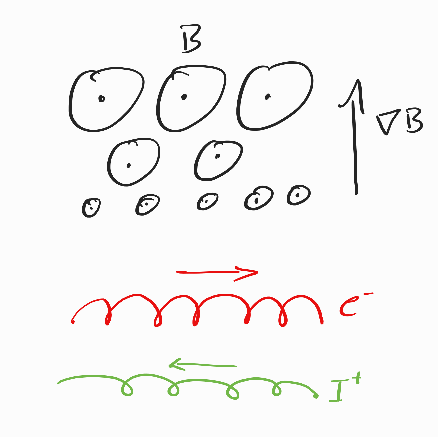
\includegraphics[scale=2.1]{imgs/c2/gradb-drift.png}
    \caption{Circles with dots indicate the magnetic field $\vec{B}$ is orientated into the page. This shows the effect of 
    $\grad \vec{B}$ drift on oppositely charged particles.}
\end{figure}\newpage

% 2.3.1.
\subsection{Generation}

There are a number of mechanisms by which runaway electrons can be generated in a tokamak.

The simplest case is one we induce ourselves - in the warm up routine of a reactor such as ISTTOK a heating element 
is applied to the gas, which ionises it. The heating of the gas follows a Maxwellian distribution, which 
gives probability that some portion of the resulting plasma will consist of electrons which have been 
energised to relativistic states \cite{runaway-electrons}. The Maxwellian distribution for electron energy densities 
can be given:
$$f_{M}(v) = \frac{n}{\sqrt{\pi} v_{\text{th}}} e^{-\frac{v^2}{v_{\text{th}}^2}}$$
where $v_{text{th}}$ describes the barrier for an electron being described thermal or not, and $n$ is the number 
of electrons present. Velocities past this barrier are referred to as being in the ``hot tail'', and are considered 
candidates for being runaway. Using this we can define an electric field for which all thermal electrons will be 
accelerated into becoming runaway electrons:
\begin{definition}[Dreicer field]
    A Dreicer field is an electric field for which all thermal electrons, defined to have at least velocity $v_{\text{th}}$,
    will be accelerated into runaway electrons.
    \begin{equation*}
        E_{D} = \frac{4\pi e^3 n \ln (\Lambda)}{m v_{\text{th}}^2}
    \end{equation*}
\end{definition}
The heating element which is the causation of this is affectionately titled a ``heating lamp'', 
though one should likely hesitate to leave it on after you go to bed. As such, no matter our efforts in dampening 
REs, and in eliminating other processes which generate them, we will necessarily have some background population 
of runaway electrons. Notably, this will also increase in magnitude for reactors which have longer 

A connected idea to this is that of runaway avalanches. If a collision takes place within the plasma between a high 
energy electron and another particle, then an avalanche can occur if that collision results in the production of another 
high energy (relativistic) electron. This avalanche effect is characterised by an exponential growth, which can be given:
\begin{equation*}
    \ln \frac{n_{\text{re}}}{n_{\text{seed}}} = \frac{e}{m_e \ln \Lambda} \frac{\Delta \psi / (2\pi R)}{\sqrt{5 + Z_{\text{eff}}}}
\end{equation*}
where $n_{\text{re}}$ is the number of resulting relativistic electrons, $n_{\text{seed}}$ describes the 
number of incident runaway electrons, and $Z_{\text{eff}}$ describes the effective background ion charge. Note that ISTTOK observes a 
presence of these ``seed'' runaway electrons after a ramp-down \cite{malaquias-matthew}.

Another contibution is that of magnetic field topolgy. When there are ``breaks'' in the magnetic field line topology that form, 
electrons within the influence of these breaks can be accelerated to relativistic speeds. While the dynamics of this are more 
complicated than simply ``topology changes, runaway electrons generated'', the occurrence of such a change in topology can be 
considered a type of runaway electron generation, and can be used to infer / support their generation if observed \cite{runaway-electrons}.
This change in topolgy could, for example, be characterised by the formation of an ``X-point'', which is a point at which two previously 
distinct magnetic field regions join together to share a single point of flux density in common, which mathemtically presents as 
a singularity, though physically acts as an unstable accelerator.


% 2.3.2.
\subsection{Detection}

It's all well and good to be know that runaway electrons are a possibility, but equally as important is being able 
to identify if you actually have runaway electrons. Unfortunately, we cannot just ask the plasma. As such, we must resort 
to a series of clever tricks to infer the existence of REs. 

The first and most obvious of these tricks is to recall that, being electrons that are moving, RE populations form a current. As 
we are able to measure current density profiles in our reactors, if we do so and observe there to be a significant, unexpected increase in 
current density, we could infer that this is the consequence of an RE population. 

\todo

$v_{\text{loop}}$ spikes 

Hard x-rays 

\begin{figure}[h!]
    \centering
    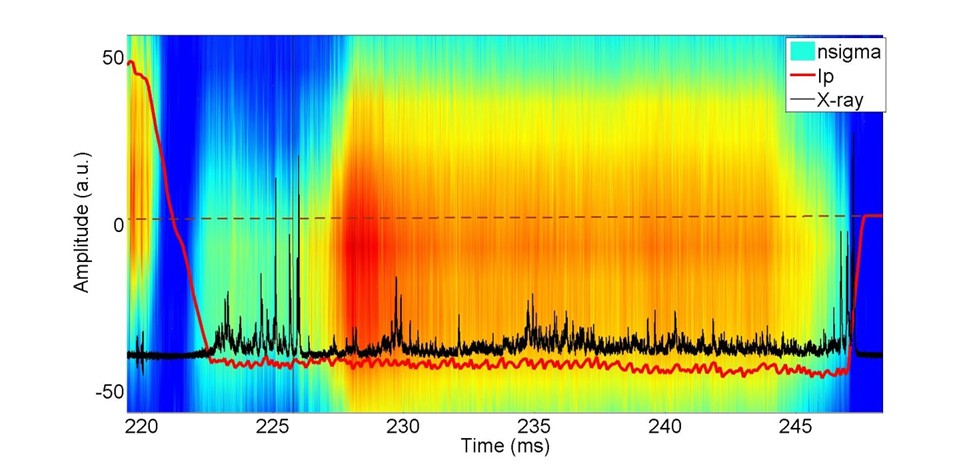
\includegraphics[scale=0.9]{imgs/c2/re-presence.png}
    \caption{ISTTOK plasma pressure density profile with plasma current ($I_p$) and X-rays detected. As X-rays are 
    an indicator of runaway electrons, this indicates an jump in RE presence during the ramp down phase, and also 
    at the start of the next ramp up phase \cite{malaquias-matthew}.}
\end{figure}


Plasma density fluctuation

Notable instrument limitation: some sensors are directional in reactor (such as x-ray detector), which means 
they can only track half the AC cycles, as half will travel in the wrong direction.